\chapter{Related Works}
\label{chapter:related_works}

\begin{introduction}
    Many authors have tackled the problem of estimating the energy consumption of parts of the \ac{ict}. However, very few have tried to estimate the energy consumption of the \ac{ict} as a whole. To make sure that the most appropriate models are used in this thesis, a review of the most recent studies was made. This review includes the criteria for selecting these models, a description on how the models work and the system boundary they act upon, and the pitfalls and assumptions of each model.
\end{introduction}

\section{Systematic review methodology}

The search methodology focused on studies that analyze energy or carbon consumption of parts of the \ac{ict} sector, such as datacenters. The search was based primarily on English language publications, using bibliographic databases such as \href{https://ieeexplore.ieee.org}{IEEE Xplore Digital Library}, \href{https://www.researchgate.net/}{ResearchGate}, \href{https://dl.acm.org/}{ACM Digital Library} and \href{https://scholar.google.com/}{Google Scholar}. Also, to complement the search we used \href{https://www.connectedpapers.com/}{ConnectedPapers}, a tool that uses the references of a paper to create a graph of papers similar to the reference.

The search was based on primarily done by using a keyword related to the specific area of the \ac{ict} sector in study followed by a keyword related to energy consumption. For example a search for datacenters would be done by using the keywords \textit{"datacenter"} and \textit{"power consumption"}. The search filtered articles to include only those above January 2000. 
From the results gathered papers that showed bottom-up models were privileged over top-down models. 

\section{Energy consumption studies}

In this section, we will present the most relevant studies gathered by the methodology described in the previous section. Each study tackles a different subsystem, however, their boundary delimitation can overlap with others, so we will frame the boundaries of the studies into the system boundaries that we have defined in \ref{section:system_boundaries}.

The methodology used by each study is different, however all use a combination of direct measurements and modeling to estimate the energy consumption of the subsystems. 

There exist several models for parts of the \ac{ict} sector, table \ref{table:energy_models} showcase the models that we will describe in this section.

\begin{table}
\caption{Bottom-up energy models and their system boundaries according to the ones defined in \ref{section:system_boundaries}.}
\label{table:energy_models}
\begin{center}
    \begin{tabular}{|| c | c | c | c | c | c ||}
        \hline
        \multirow{2}{*}{Study} & \multirow{2}{*}{Year of data} & \multicolumn{4}{c||}{System Boundary} \\ \cline{3-6}
        & & \ac{cpe} & \ac{an} & Core Network & Datacenter \\
        \hline
        \citet{Coroama2015} & 2 & \checkmark & \checkmark &  &   \\ \hline
        \citet{Baliga2009} & 2 & \checkmark & \checkmark & \checkmark &   \\ \hline
        \citet{Schien2015} & 2 &  &  & \checkmark &   \\ \hline
        \citet{Taal2014} & 2 &  &  & \checkmark & \checkmark  \\ \hline
        \citet{USReport2016} & 2 &  &  &  & \checkmark  \\ \hline
        \citet{Li2014} & 2 &  &  &  & \checkmark  \\ \hline
    \end{tabular}
\end{center}
\end{table}

%% Coroama 2015

\citet{Coroama2015} uses both approaches to estimate the energy consumption of the \ac{cpe} and access network subsystems. They developed a formula, (\ref{formula:coroama_cpe_an}), for estimating the energy intensity of these two subsystems. The formula builds on their previous analysis of multimedia servers \citet{Schien2013}. The formula is as follows: 

\begin{equation}
\label{formula:coroama_cpe_an}
    I_{CPE,AN} = \frac{t_{on}}{t_{use}} \frac{P_{CPE}}{N_{CPE}} + \frac{P_{AN}}{N_{AN}} PUE_{AN}.
\end{equation}

Where: 

\begin{itemize}
    \item $I_{CPE,AN}$: Intensity of both \ac{cpe} and \ac{an}.
    \item $\frac{t_{on}}{t_{use}}$: Ratio of time that the device is actively working. 
    \item $P_{CPE}$: Power of all \ac{cpe} devices.
    \item $N_{CPE}$: Number of Users connected to the \ac{cpe}.
    \item $P_{AN}$: Power of all \ac{an} devices.
    \item $N_{AN}$: Number of users (subscribers) connected to the \ac{an}.
    \item $PUE_{AN}$: \ac{pue} of the \ac{an}.
\end{itemize}

$\frac{P_{AN}}{N_{AN}}$ gives the energy intensity of the \ac{an} per subscriber, the technology they evaluate is \ac{adsl}2 which has a power consumption of \SI{2}{\watt} per subscriber \citet{Schien2013}. As for the $PUE$ they assume a value of 2. 
$\frac{P_{CPE}}{N_{CPE}}$ gives the energy intensity of the \ac{cpe} per subscriber. The study assumes that each household has 2 \ac{cpe} devices, a modem and a router, and arrives at a value of \SI{8}{\watt} per subscriber when accounting for legacy equipment. 
The ratio of time that the device is actively working is estimated to be 6 according to the findings in \citet{Nissen2007}.
The study then concludes that the energy intensity for this subsystem is \SI{52}{\watt} per subscriber.

%% Baliga 2009

\citet{Baliga2009} evaluates the impact of different \ac{ip} technologies, and uses data from manufacture data sheets to supplement its assumptions. They use a simple model (\ref{formula:baliga_cpe_an}) to estimate the energy consumption of the \ac{cpe} and \ac{an} subsystems and evaluate different technologies such as \ac{adsl}, \ac{pon}, \ac{fttn} and \ac{ptp}. The model is as follows:  

\begin{equation}
\label{formula:baliga_cpe_an}
    P_a = P_{CPE} + \frac{P_{RN}}{N_{RN}} + \frac{2P_{TU}}{N_{TU}}
\end{equation}

\begin{itemize}
    \item $P_a$: Power consumption of the \ac{cpe} and \ac{an} subsystems.
    \item $P_{CPE}$: Power consumption of the \ac{cpe}.
    \item $P_{RN}$: Power consumption of the remote node.
    \item $N_{RN}$: Number of subscribers that share remote nodes.
    \item $P_{TU}$: Power consumption of the terminal unit at the central office.
    \item $N_{TU}$: Number of subscribers that share  terminal units.
    \item The factor of 2 corresponds to the \ac{pue}.  
\end{itemize}

For the core network specifications from Cisco CRS-1 core routers were used to develop a per costumer power consumption model (\ref{formula:baliga_core}):

\begin{equation}
\label{formula:baliga_core}
    P_c = \frac{8A_{T}(H + 1)}{640 Gbps} \cdot \SI{10.9}{\kilo\watt}
\end{equation}

With: 

\begin{itemize}
    \item $P_c$: Power consumption of the core network.
    \item $A_{T}$: Minimum capacity available to a customer.
    \item $H$: Number of core node hops.
    \item The factor of 8 accounts for the fact that core routers are usually provisioned for future growth of double the current peak demand, to account for redundancy and \ac{pue}.
\end{itemize}

%% Schien 2015
 
\citet{Schien2015} developed a model for the subsystem of core network. The study created a model to estimate the energy consumption of data traffic in the core network, that is the cost per \ac{gigabyte} of data transmitted. 
The model only considers the devices that will carry the connection data between the user and the server. Because not all energy spent by each device is directly related to a request, the energy intensity is the ratio between the energy spent by the device and the data throughput. The study distinguish between metro and long-haul networks, and use similar models for both. The model for the metro network is as follows:

\begin{equation}
\label{formula:schien_core_metro}
    I_{M_{TM}} = R \cdot n_{M_R} (c_{ON} \cdot I_{ON} + n_{M_{OA}} \cdot I_{OA})
\end{equation}

Where:

\begin{itemize}
    \item $R$: Redundancy.
    \item $n_{M_R}$: Number of metro routers.
    \item $c_{ON}$: Ratio of \ac{wdm} systems relative to routers.
    \item $I_{ON}$: Energy intensity per \ac{wdm} system.
    \item $n_{M_{OA}}$: Number of metro network optical amplifiers per hop.
    \item $I_{OA}$: Energy intensity per metro network optical amplifier.
\end{itemize}


%% Taal2014

Another model for the core network was developed by \citet{Taal2014}. The study models the energy consumption of offloading data between datacenters, so it includes in  its analysis the energy consumption of data being stored in datacenters as well as the cost of transmitting the data through the network. 
The study analysis the possibility of data to travel through public internet or by a dedicated network called \textit{lightpath}. The difference between the two is that the \textit{lightpath} does not need routing therefore the \ac{dwdm} nodes are directly connected to each other, whilst in the public internet the \ac{dwdm} nodes are connected to routers and switches. Figure \ref{figure:tall2014_network_components} shows the difference between the two networks. The energy consumption is defined as a function of data passing through the network ($D_{in}$). The models for the public internet and \textit{lightpath} are as follows:

\begin{figure}[h] 
    \centering
    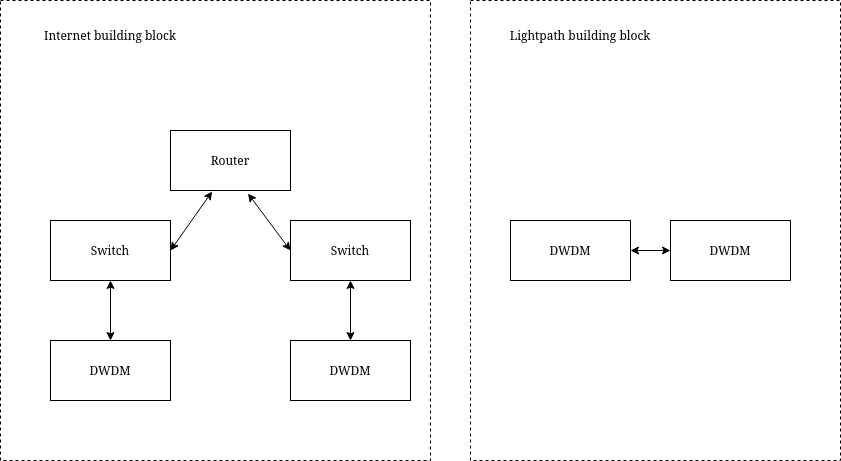
\includegraphics[width=0.8\textwidth]{figs/taal2014.png}
    \caption[Network components of the internet and \textit{lightpath}] {Network components of the internet and \textit{lightpath}, on the left it showcases the internet building blocks composiong of 2 \ac{dwdm} nodes, 2 switches and 1 router. On the right it showcases the \textit{lightpath} building blocks, composed of 2 \ac{dwdm} nodes. Figure adapted from \citet{Taal2014}.}
    \label{figure:tall2014_network_components}
\end{figure}
 
\begin{equation}
\label{formula:tall_public_internet}
\begin{split}
    E_{internet}(D_{in}) = & \frac{PUE_{network}}{U} \cdot \frac{8D{in}}{3600} \cdot \\
    \Bigg( \bigg( \frac{2P_{switch}}{C_{switch}} + \frac{2P_{DWDM}}{C_{DWDM}} \bigg) + \bigg(\frac{2P_{switch}}{C_{switch}} & + \frac{2P_{DWDM}}{C_{DWDM}} + \frac{P_{router}}{C_{router}}\bigg) \cdot n_{hops} \Bigg)
\end{split}
\end{equation}

\begin{equation}
\label{formula:tall_lightpath}
\begin{split}
    E_{lightpath}(D_{in}) = & \frac{PUE_{network}}{U} \cdot \frac{8D{in}}{3600} \cdot \\
    \Bigg( \bigg( \frac{2P_{switch}}{C_{switch}} + \frac{2P_{DWDM}}{C_{DWDM}} \bigg) + \bigg(\frac{2P_{DWDM}}{C_{DWDM}}\bigg) \cdot n_{hops} & + \bigg( \frac{P_{switch}}{C_{switch}} \bigg) \cdot \bigg( n_{hops} - 1 \bigg) \Bigg)
\end{split}
\end{equation}

Where:

\begin{itemize}
    \item $PUE_{network}$: \ac{pue} of the network.
    \item $U$: Utilization of the network.
    \item $P_{switch}$: Power of the switch.
    \item $C_{switch}$: Capacity of the switch.
    \item $P_{DWDM}$: Power of the \ac{dwdm} node.
    \item $C_{DWDM}$: Capacity of the \ac{dwdm} node.
    \item $P_{router}$: Power of the router.
    \item $C_{router}$: Capacity of the router.
    \item $n_{hops}$: Number of hops between the datacenters.
\end{itemize}

As for the estimation of the energy consumption of the datacenter, the study considers 3 costs, the cost of writing data ($E_{write}$), reading data ($E_{read}$) and the cost of storing data ($E_{store}$). The study assumes a \ac{san} consisting of a content server, an Ethernet switch and a storage array of several disks. The equations for each cost are expressed below:

\begin{equation}
\label{formula:tall_datacenter_write}
    E_{write}(D_{in}) = \frac{PUE}{U} \cdot \frac{8D_{in}}{3600} \cdot \bigg(\frac{P_{server}}{C_{server}} + \frac{P_{sw}}{C_{sw}} + N_d(D_{in}) \frac{P_{disk}}{C_{disk}}  \bigg) 
\end{equation}

Where:
\begin{itemize}
    \item $PUE$: \ac{pue} of the datacenter.
    \item $U$: factor that accounts for the utilization of the data equipment, expressing the fact data equipment typically does not operate at a full utilization while still consuming 100\% of the power, $U = 0.5$.
    \item $\frac{8D_{in}}{3600}$: convertion of Gbps to GBph
    \item $P_x$: power consumption in kW of server, switch and disk.
    \item $C_x$: capacity of the server, switch and disk.
    \item $N_d(D_{in})$: function of the number of disks used for capacity $D_{in}$, assuming a configuration of RAID 10, given by: 
\end{itemize}

\begin{equation}
\label{formula:tall_datacenter_ndisks}
    N_d(D_{in}) = 2 \cdot \bigg \lceil \frac{D_{in}}{S_{array} \cdot S_{disk}} \bigg \rceil
\end{equation}

\begin{itemize}
    \item $S_{array}$: Number of disks in the array
    \item $S_{disk}$: Capacity of disks (GB)
\end{itemize}

\begin{equation}
\label{formula:tall_datacenter_store}
    E_{store}(D_{in}, RT) = \frac{PUE}{U} \cdot N_d(D_{in}) \cdot P_{disk} \cdot RT
\end{equation}

\begin{itemize}
    \item $RT$: retention time of the data stored
\end{itemize}

\begin{equation}
\label{formula:tall_datacenter_read}
    E_{read}(D_{out}) = \frac{PUE}{U} \cdot \frac{8D_{out}}{3600} \cdot \bigg(\frac{P_{server}}{C_{server}} + \frac{P_{sw}}{C_{sw}}  \bigg)
\end{equation}

\begin{itemize}
    \item $D_{out}$: Data being read.
\end{itemize}

%% US Report 2016

\citet{USReport2016} developed a model for the subsystem of datacenters. The report evaluates the yearly consumption of datacenters in the US until 2014 and forecasts the consumption until 2020. Data from \ac{idc} was collected to determine the installed base, in terabytes (\SI{}{\tera\byte}), per type of disk (\ac{hdd}, \ac{ssd}) and their information of previous report \citet{USReport2007} was used to convert the installed based to \SI{}{\tera\byte}/drive.
Electricity consumption is calculated as the product of the estimated installed base of drives and the assumed power consumption per drive.

\begin{equation}
\label{formula:usreport2016}
    E_y = \sum_{t=HDD,SSD}{(I_{t,y} * P_{t,y}) * h_y * (1 + O * \frac{C_{external}}{C_{total}})}
\end{equation}

Where:

\begin{itemize}
    \item $E_y$: Storage electricity consumption in year y
    \item $I_{t,y}$: Installed base of storage type t in year y
    \item $P_{t,y}$: Per-unit power consumption of storage type t in year y
    \item $h_y$: Number of hours in year y
    \item $O$: Operational energy as a fraction of storage energy
    \item $C_{external}$: Capacity of the external storage installed base
    \item $C_{total}$: Capacity of the total storage installed base
\end{itemize}

The second part of the equation $(1 + O * \frac{C_{external}}{C_{total}})$ refers to the operational cost of storage that is external to the server.
The report states that operational cost is assumed to be 25\% of the storage energy, based on industry comment, and it only applies to external storage.

%% Li Y

\citet{Li2014} studied the energy cost of I/O workloads. According to the paper, the power consumption of storage devices such as \ac{hdd} and \ac{ssd} is dependent on the workload type, which can be either capability or capacity. Capability workloads are when its demand for I/O bandwidth is more difficult to meet than its demand for storage space. For example a web server. Capacity is when the requirement for storage space is greater than other requirements. The paper also takes into account power saving techniques that disk may implement, so it differentiates between active and idle power consumption. However, This approach doesn't take into account the operational and cooling costs.
The formula for calculating the energy consumption of the I/O operation:

\begin{equation}
    E = T_a P_i N_i + T_a P_b N_a
\end{equation}
Where:

\begin{itemize}
    \item $E$: Energy consumption of the workload.
    \item $T_a$: The time needed to complete the workload.
    \item $P_i$: Power consumption  of the device in idle mode.
    \item $N_i$: The number of idle devices during the workload.
    \item $P_b$: Power consumption of the device in active mode.
    \item $N_a$:The number of active devices during the workload.
\end{itemize}

The $T_a$ can be expressed as: 

\begin{equation}
    T_a = \frac{W_c}{W_{ab}}
\end{equation}
With:
\begin{itemize}
    \item $W_c$: Workload capacity requirement.
    \item $W_{ab}$: Workload average bandwidth requirement.
\end{itemize}

Given that the total number of devices ($N$) is equal to the sum of the number of idle devices ($N_i$) and the number of active devices ($N_a$), they determine the number of active and idle devices with the formulas below:

\begin{equation}
    N = \left \lceil {\frac{W_c}{D_c}} \right \rceil
\end{equation}
\begin{equation}
    N_a = \alpha \frac{W_{ab}}{D_b}
\end{equation}
\begin{equation}
    N_i = N - N_a
\end{equation}

\begin{itemize}
    \item $W_c$: Workload capacity requirement.
    \item $W_{ab}$: Workload average bandwidth requirement.
    \item $D_c$: Device capacity.
    \item $D_b$: Device bandwidth.
    \item $\alpha$: if $N_{min}$ is the theoretical minimum number of devices needed to complete the workload then, $\alpha N_{min}$ is the actual number of devices needed, $\alpha \in [1,\frac{N}{N_{min}}]$.
\end{itemize}


% \subsection{Direct measurement}

% Another approach is to directly measure the power consumption and data traffic of equipment within a network. These model use the data collected to extrapolate the energy consumption of each component of the network and are able to forecast the energy consumption of the network.

% %% Maldomin 2010

% \citet{Malmodin2010} focus on the Sweden \ac{ict} sector and uses both top-down data collection of traffic and energy measurements of several network sites, and bottom-up data from user data traffic measurements and network equipment databases.  
% From their data collected they extrapolate the energy consumption of the \ac{ip} core network at \SI{126}{\giga\watt\hour}

% %% Krug 2014

% \citet{Krug2014} used data from 2012 of the BT UK network, a major supplier of telecommunications services in the UK. The study presents a metric called "energy per bit" that is calculated as: the
% power per line multiplied by the number of seconds in a month divided by the bits per line in a month. 